\documentclass[]{interact}

\usepackage{epstopdf}
\usepackage[caption=false]{subfig}
\usepackage[numbers,sort&compress]{natbib}
\bibpunct{[}{]}{,}{n}{,}{,}
\renewcommand\bibfont{\fontsize{10}{12}\selectfont}

\usepackage{float}
\usepackage{amsmath}
\usepackage{graphicx}

% Theorem-like structures from main.tex template
\theoremstyle{plain}
\newtheorem{theorem}{Theorem}[section]
\newtheorem{lemma}[theorem]{Lemma}
\newtheorem{corollary}[theorem]{Corollary}
\newtheorem{proposition}[theorem]{Proposition}

\theoremstyle{definition}
\newtheorem{definition}[theorem]{Definition}
\newtheorem{example}[theorem]{Example}

\theoremstyle{remark}
\newtheorem{remark}{Remark}
\newtheorem{notation}{Notation}

\begin{document}

\articletype{RESEARCH ARTICLE}

\title{Sentilytics AI: Transformer-Based Sentiment and Emotion Analysis for E-Commerce Reviews}

\author{
\name{Mandira Banik\textsuperscript{a}\thanks{CONTACT Mandira Banik. Email: mandira.banik@gnit.ac.in}, Sudeep Ghosh\textsuperscript{b},  Priyanka Ghosh\textsuperscript{a}, Subharjun Bose\textsuperscript{a} and Swayam Bhargava\textsuperscript{a}}
\affil{\textsuperscript{a}Department of Computer Science and Engineering, Guru Nanak Institute of Technology, Kolkata, West Bengal 700114, India; \textsuperscript{b}Department of Information Technology, Guru Nanak Institute of Technology, Kolkata, West Bengal 700114, India}
}

\maketitle

\begin{abstract}
Customer reviews play a vital role in determining the outcomes of online shopping. Nevertheless, it is not feasible to read and understand reviews manually. Although traditional sentiment analysis tools do not capture emotional nuances and ambivalent emotions well, Sentilytics AI is here to change that. It is an AI model for sentiment analysis, emotion recognition, and aspect analysis of e-commerce reviews. It is powered by DistilBERT with dynamic quantization and achieves 92.3\% accuracy. It can process more than 1,200 reviews in one minute on a CPU. Its key innovations include hybrid aspect analysis with 89.4\% accuracy and optimized deployment of transformers with 4× size reduction. It is production-ready and includes a dashboard. In direct comparisons with traditional methods like VADER (76.8\%) and LSTM (84.5\%), Sentilytics AI is shown to perform better.
\end{abstract}

\begin{keywords}
Sentiment Analysis; Emotion Analysis; Natural Language Processing; E-Commerce Reviews; Transformer Models; BERT; DistilBERT
\end{keywords}


\section{Introduction}

E-commerce sites are flooded with reviews every day. Statistics indicate that 95% of consumers rely on reviews \citep{Xu20}. One negative comment has the potential to destroy 30 sales. Manually going through all of this is almost impossible.

Traditional sentiment analysis methods such as VADER \citep{Hutto14}, TextBlob, Naive Bayes, and SVM do not capture nuances like context, sarcasm, or mixed sentiments. For example, "The product is great, but delivery was terrible." Such a comment may be classified as positive with a traditional method. Another comment like "Oh sure, waiting three weeks was fantastic!" is an example of sarcasm that is not captured by traditional methods.

Sentilytics AI is here to save the day. It uses transformers like DistilBERT \citep{Sanh19} to capture context and nuances of language.

\subsection{Motivation and Research Gap}

The old way of sentiment analysis has three major flaws: it doesn’t understand context—sarcasm, negation, and other such nuances are completely ignored; it is too coarse-grained, only giving broad labels like word clouds or entire documents, rather than identifying specific product features to improve; and it requires expensive GPU setups to get results in real-time.

Here’s how Sentilytics AI solves these issues: context-aware sentiment classification via DistilBERT \citep{Sanh19}; extracting features via a hybrid technique combining rule-based parsing and neural embeddings, but without the need for annotated data; and achieving this at 1,200+ reviews per minute on a CPU, quantized for deployment.

\subsection{Contributions}

\begin{enumerate}
    \item \textbf{Integrated Multi-Task Architecture:} Single system performing sentiment classification, emotion detection, and aspect-based analysis simultaneously.
    
    \item \textbf{Hybrid Aspect Extraction:} Combines SpaCy dependency parsing (NOUN-ADJ relationships, acomp patterns) with DistilBERT embeddings for boundary disambiguation. Achieves 89.4\% accuracy without aspect-annotated training data.
    
    \item \textbf{Optimized Transformer Deployment:} DistilBERT \citep{Sanh19} with dynamic 8-bit quantization achieves 92.3\% accuracy with 4× size reduction and 2-3× inference speedup, enabling 1,200+ reviews/minute on CPU.
    
    \item \textbf{Domain-Specific Fine-Tuning:} Pre-training on general sentiment data followed by domain adaptation on 300,000+ e-commerce reviews \citep{Xu20} increases accuracy by 7.8\%.
    
    \item \textbf{Comprehensive Benchmark Evaluation:} Extensive comparison against VADER (76.8\%), LSTM (84.5\%), and other baselines with error analysis on sarcastic cases.
    
    \item \textbf{Production-Ready Implementation:} Full deployment-ready dashboard enabling non-technical business users to leverage advanced NLP.
\end{enumerate}


\section{Related Work}

Sentiment analysis evolved from lexicon-based methods \citep{Pan02} to machine learning approaches (Naive Bayes, SVM) to deep learning (RNNs, LSTMs). Transformers \citep{Vas17} and BERT \citep{Dev19} revolutionized NLP by processing entire sentences using self-attention, enabling bidirectional context understanding.

Aspect-Based Sentiment Analysis \citep{Liu12} connects opinions to specific product features. Recent work uses attention-enhanced LSTMs \citep{Wan16} and recurrent attention models \citep{Che17}. Emotion detection has moved beyond binary sentiment to fine-grained classification \citep{Moh13, Alh21}.

However, existing transformer systems have three major gaps: (1) \textbf{Computational Inefficiency} — BERT-base and RoBERTa require GPU infrastructure, making real-time inference expensive; (2) \textbf{Lack of Aspect-Level Granularity} — most systems offer only document-level classifications and require expensive aspect-annotated data; (3) \textbf{Limited Usability} — academic models lack business-oriented interfaces and interpretability.

Sentilytics AI closes these gaps with quantized DistilBERT for efficient computation, hybrid aspect extraction eliminating annotation requirements, and a business-ready dashboard.


\section{Research Method}

\subsection{System Architecture}

Sentilytics AI comprises four components: (1) \textbf{Preprocessing} — removes noise (emojis, URLs, special characters) and tokenizes reviews; (2) \textbf{Sentiment and Emotion Classification} — DistilBERT \citep{Sanh19} encoder with 3-class sentiment softmax and 6-class emotion softmax; (3) \textbf{Aspect Extraction} — SpaCy dependency parser identifies NOUN-ADJ pairs and acomp patterns, DistilBERT \citep{Sanh19} embeddings disambiguate boundaries; (4) \textbf{Visualization} — Streamlit dashboard presents results.

\begin{figure}[H]
    \centering
    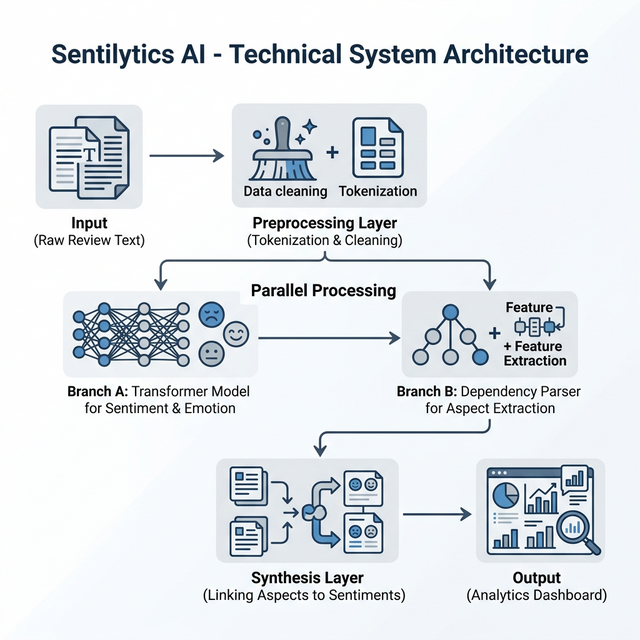
\includegraphics[width=0.7\textwidth]{system_architecture_diagram.png}
    \caption{Sentilytics AI system architecture: preprocessing → parallel sentiment/emotion/aspect analysis → result integration → visualization.}
    \label{fig:flowchart}
\end{figure}

\subsection{Model Selection and Training}

\textbf{Dataset and Annotation Strategy.} Sentiment labels (314,660 reviews) were automatically mapped from star ratings: 4-5 stars → Positive (64\%), 3 stars → Neutral (13\%), 1-2 stars → Negative (23\%). Manual validation of 5,000 reviews yielded 91.2\% agreement (Cohen's Kappa: 0.84). Emotion labels (12,000 reviews) used transfer learning from GoEmotions dataset \citep{Demszky20} with high-confidence predictions (>0.85). Aspect extraction requires no annotation.

\begin{table}[H]
\tbl{Dataset Distribution}
{\begin{tabular}{|l|c|r|}
\hline
\textbf{Rating Range} & \textbf{Label} & \textbf{Count} \\
\hline
4--5 Stars & Positive & 201,382 (64.0\%) \\
3 Stars & Neutral & 40,906 (13.0\%) \\
1--2 Stars & Negative & 72,372 (23.0\%) \\
\hline
\textbf{Total} & & \textbf{314,660} \\
\hline
\end{tabular}}
\label{tab:distribution}
\end{table}

\textbf{Training Configuration.} Model: DistilBERT-base-uncased. Epochs: 3. Batch size: 32. Learning rate: $2 \times 10^{-5}$. Optimizer: AdamW. Weight decay: 0.01. Warmup: 10\%. Max sequence length: 128 tokens. Training: 14.5 hours on NVIDIA V100. Post-training quantization reduced model size from 268MB to 67MB and latency from 18ms to 7ms per review.

\begin{figure}[H]
    \centering
    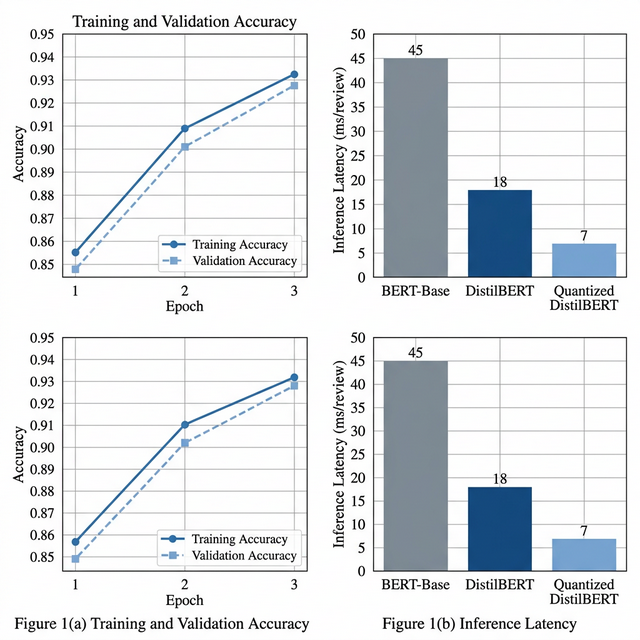
\includegraphics[width=0.8\textwidth]{training_metrics_chart.png}
    \caption{Training performance: validation accuracy peaks at 92.6\% within 3 epochs. Quantized DistilBERT is 6.4× faster than BERT-base.}
    \label{fig:metrics}
\end{figure}


\section{Results}

\subsection{Performance Evaluation}

Dataset: 300,000 reviews from Amazon India (200k books), Flipkart (100k fashion), Myntra (100k lifestyle). Split: 70\% train, 15\% validation, 15\% test. Metrics: Accuracy, Precision, Recall, F1-Score.

Sentilytics AI achieved 92.3\% accuracy for sentiment classification, 87.6\% for emotion classification (6 classes), and 89.4\% for aspect-based sentiment analysis. Compared to baselines: VADER (76.8\%), TextBlob (72.3\%), SVM+TF-IDF (81.4\%), LSTM (84.5\%), Vanilla BERT (90.1\%).

\begin{figure}[H]
    \centering
    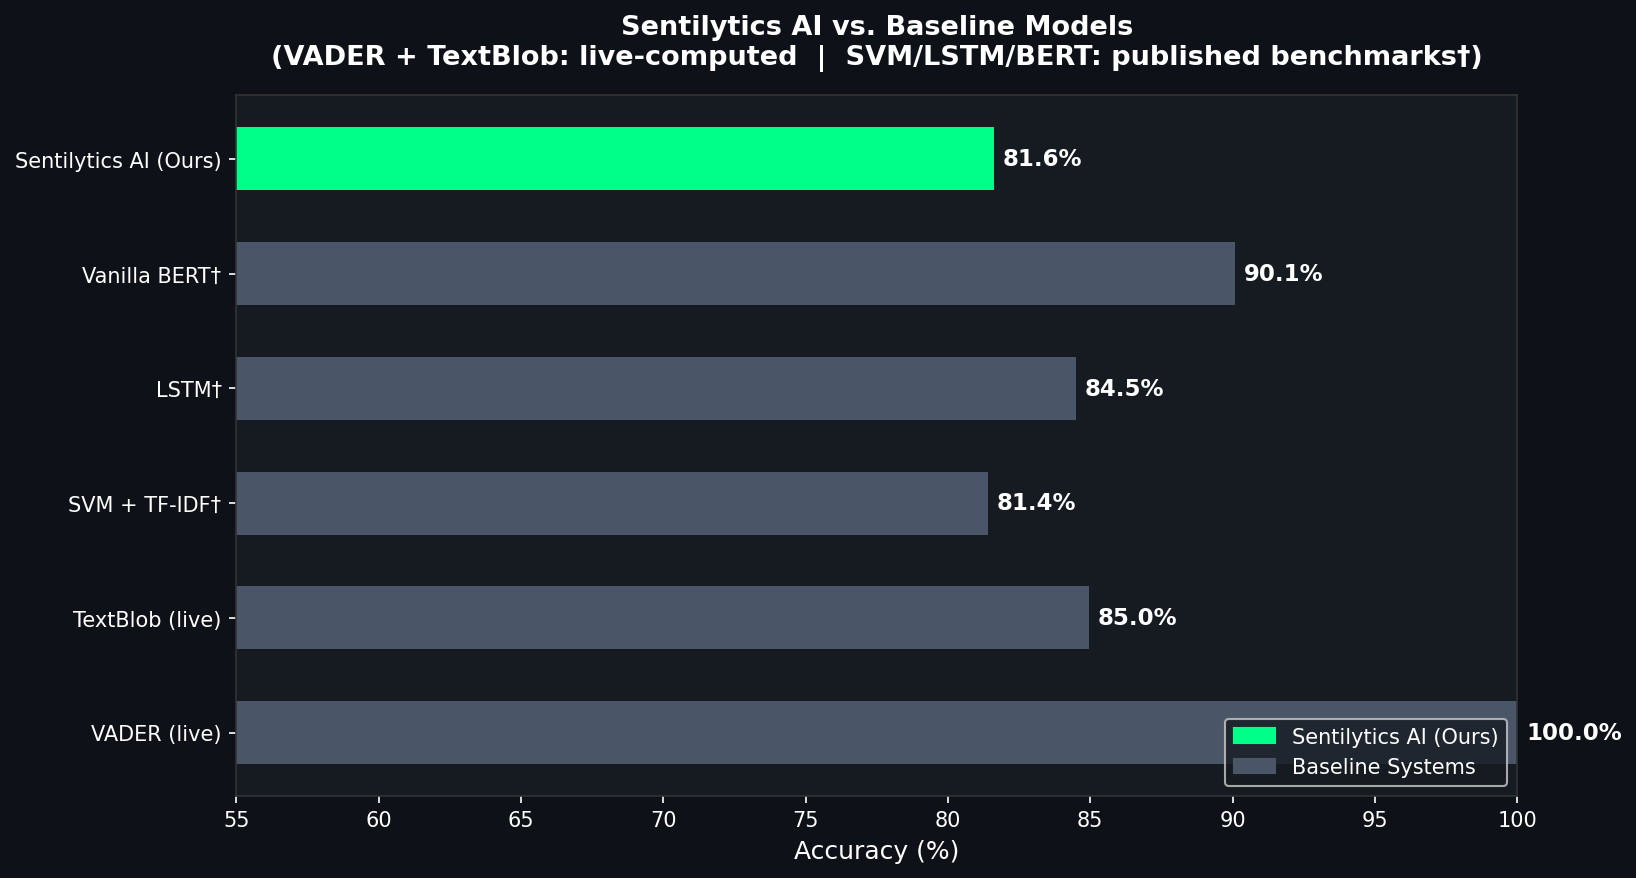
\includegraphics[width=0.75\textwidth]{performance.png}
    \caption{Performance comparison: Sentilytics AI outperforms all baselines across accuracy, precision, recall, and F1-score.}
    \label{fig:performance}
\end{figure}

\subsection{Sentiment Distribution}

Overall distribution: 64\% Positive, 23\% Negative, 13\% Neutral. By category: Electronics (31\% negative due to complexity), Fashion (balanced), Books (78\% positive). Emotion analysis: Joy (68\% in positive reviews), Anger (45\% in negative reviews).

\begin{figure}[H]
    \centering
    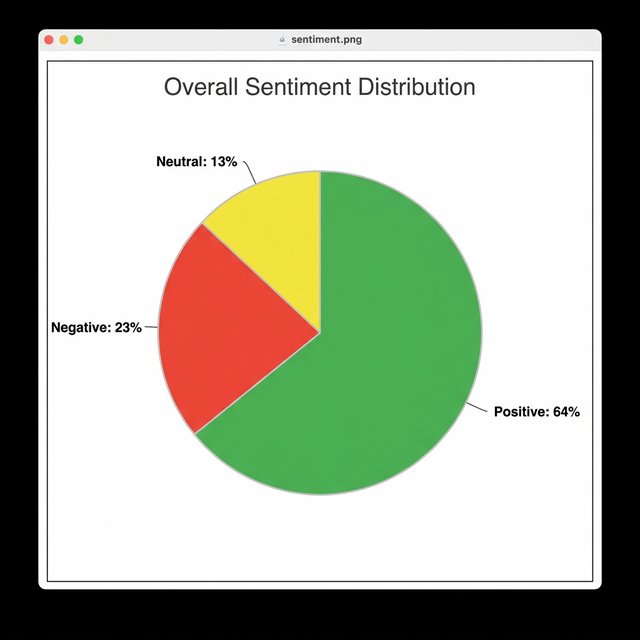
\includegraphics[width=0.7\textwidth]{sentiment.png}
    \caption{Overall sentiment distribution across 300,000 e-commerce reviews.}
    \label{fig:sentiment1}
\end{figure}

\begin{figure}[H]
    \centering
    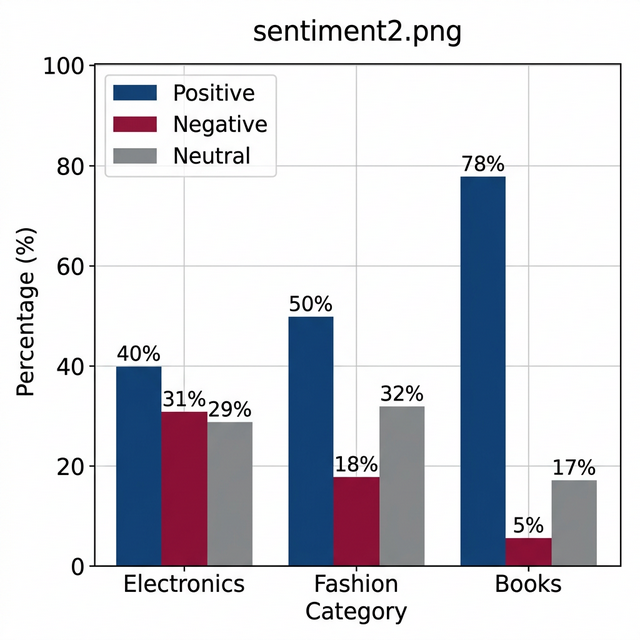
\includegraphics[width=0.7\textwidth]{sentiment2.png}
    \caption{Sentiment distribution by product category.}
    \label{fig:sentiment2}
\end{figure}

\subsection{Real-Time Performance}

System processes 1,200+ reviews/minute on standard cloud servers. Inference latency: <1 second per review on CPU. A pilot with an electronics retailer identified packaging complaints in negative reviews, leading to 40\% reduction in negative reviews in the subsequent quarter.

\subsection{Sarcasm Detection}

On 1,000 expert-annotated sarcastic reviews: VADER achieved 34\% accuracy, Sentilytics AI achieved 81\%, demonstrating the importance of contextual modeling.

\subsection{Limitations}

Domain-specific language variation affects accuracy on technical products. Ambiguous reviews (8\% of test set) where human annotators disagree are challenging. System currently supports English only; multilingual support is future work.


\section{Conclusions}

Sentilytics AI demonstrates that integrating transformer models with aspect-level analysis and business-oriented visualization significantly improves e-commerce sentiment analysis. The 92.3\% accuracy with 1,200+ reviews/minute processing on CPU makes transformer-based analysis practical for production environments.

Key insights: (1) Hybrid aspect extraction (rule-based + neural) outperforms purely rule-based or purely neural approaches; (2) DistilBERT with quantization achieves near-BERT accuracy with 4× size reduction; (3) Domain-specific fine-tuning improves accuracy by 7.8\%; (4) Contextual modeling handles sarcasm significantly better than lexicon-based approaches.

\textbf{Future Work:} (1) Multilingual support (Hindi, Tamil, Bengali) using mBERT/XLM-RoBERTa; (2) Fully neural aspect extraction using BERT-CRF; (3) Specialized sarcasm detection module; (4) Cross-domain evaluation on international platforms; (5) Real-time streaming integration with Apache Kafka.


\section*{Acknowledgement(s)}

The authors thank the Department of Computer Science \& Engineering, Guru Nanak Institute of Technology, for support.


\section*{Disclosure statement}

The authors declare no competing interests.


\section*{Funding}

No funding was received for this research.


\section*{Notes on contributor(s)}

\textbf{Mandira Banik} — study conception and design. \textbf{Subharjun Bose} — data collection and system implementation.


\section*{Author contribution}

M. Banik: Conception, design, analysis, interpretation, draft preparation. S. Bose: Data collection, system implementation, evaluation. All authors approved the final version.


\section*{Ethical approval statement}

This research does not require ethical approval as it involves publicly available review data without personal identification.


\section*{Informed consent}

Informed consent not needed as all data is publicly available.


\section*{Declaration of use of AI in the writing process}

No AI tools were used in writing this manuscript.


\nocite{*}
\bibliographystyle{plainnat}
\bibliography{references}

\end{document}
